% Appendices are set up same as chapter sections
\chapter*{Appendix}
\addcontentsline{toc}{chapter}{Appendix}

\setcounter{section}{0}

\renewcommand\thesection{\Alph{section}}

\vspace{1em}
\hiddensection{Original Project Prompt}

\begin{figure}[h]
   \centering
     \includegraphics[width=0.9\textwidth]{Figures/Appendix/project_prompt}
   \caption{Original Project prompt}
   \label{fig:projectprompt}
\end{figure}

\hiddensection{Benchmarking}
\label{sec:benchmarkingAppendix}
\begin{figure}[ht]
\centering
	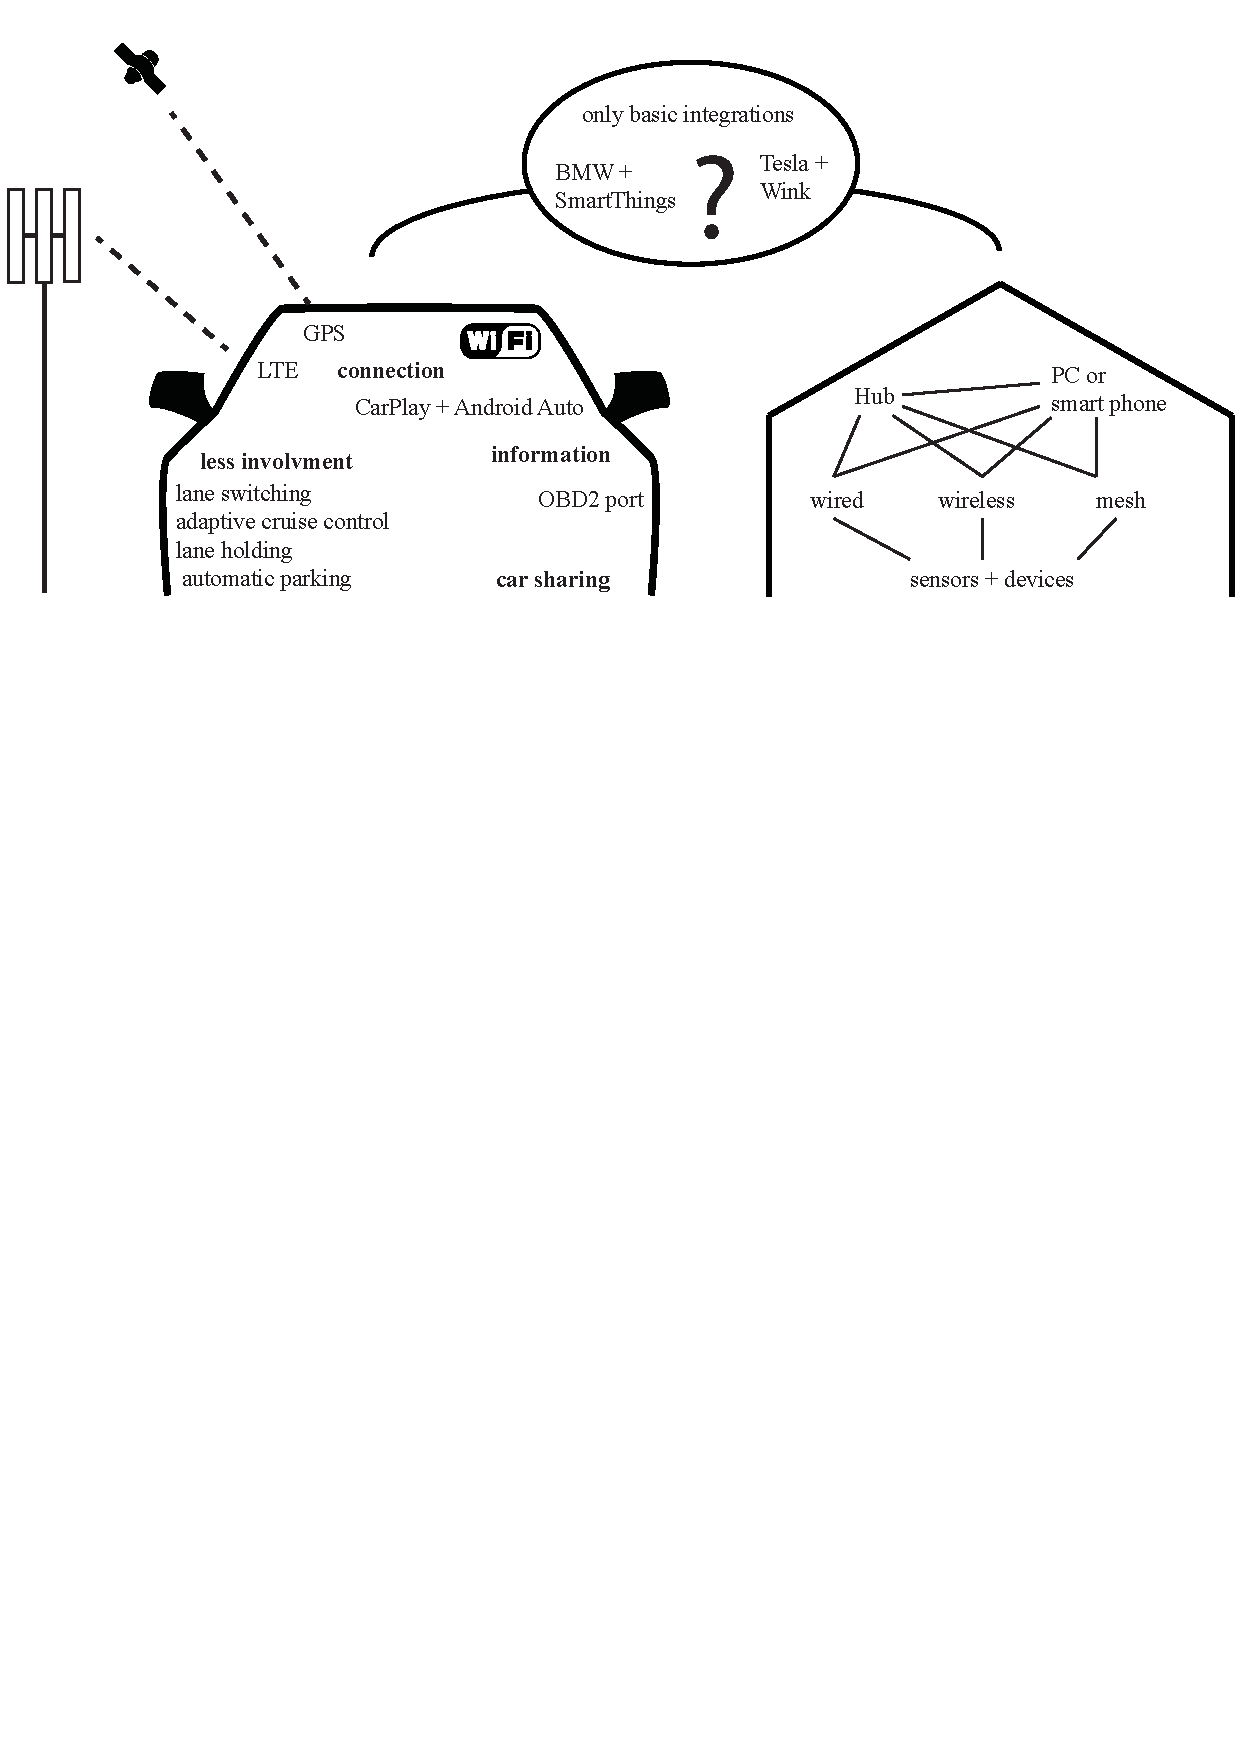
\includegraphics[keepaspectratio, width=6in]{Figures/BenchmarkingOld/benchmarking_overview.pdf}
	\caption{The smart car and smart home of today as a coarse overview}
	\label{fig:benchmarking_overview}
\end{figure}

To get an initial grasp of the problem space, we set out to explore the current state of the art as well as items of the near future. In general, we reached the conclusion that the products marketed as "smart" currently available on the market are merely automated and connected, but not really smart. 

We discovered that for us it is crucial to first define what the word "smart" in connection with home and car means. For our scenario, in the most broad sense, it could be any advanced usage of car and home, which will lead us to innumerable areas like recreation, living space, study etc. In a more widely accepted general meaning, "smart" is used to describe appliances that provide automatic and sophisticated reactions according to user input and environment sensing enabled by computing power. It is important to point out that for us this means the user should be supported and empowered by technology without having to program a routine into every device. The devices should talk with each other and keep learning and adapting to the users habits while unobtrusively staying in the background. This area is closely related to internet of things and artificial intelligence.
%% Smartness is NOT related to getting around
% As far as this project is concerned, the smartness could be any satisfactory experience of getting around that is within the physical space of home and car.

\hiddensubsection{Smart cars in the future}

One essential part of smart technology is simple driving, in which case the car manufacturers are adding value by slowly providing parts of functionality that a user would expect from a self-driving car: lane switching, lane holding and adaptive cruise control point to a future in which a driver has to be less involved. As an illustration, the adaptive cruise control is able to adjust the speed of the car to the one up front in case the car in front is driving slower than the set speed. State of the art systems can slow down up to a full stop and also start again (automatically starting again is only possible for a short time frame after stopping). Cars can also automatically park themselves, warn and brake in dangerous situations, read and notify the driver of speed limits and lane overpasses, get software updates over the internet and even switch lanes by tapping the turn signal.~\cite{TeslaAutopilot}

Modern cars have a wide variety of assisting and connecting features. Many technologies try to take over tedious tasks while driving.  Technologies like linking cell phones to the car to enable telephone features as well as entertainment options have been around for some time. Apple's CarPlay and Android Auto are technologies pushing this even further by blurring the line between phone and car by making smart phone features available on the car media system.

There are also third-party products to enhance the car into being more connected. The most interesting findings in this area for us are adapters connecting to the car's diagnostic OBD2 port, which is available in almost every car across all manufacturers. The user can then connect to the adapter via WiFi or Bluetooth and access different car related information.

The future of the automobile industry is interesting as well. There are trends like car sharing, moving away from everyone owning his personal car towards sharing one car among several people. This goes along with more and more people living in big cities where there is not such a need for a private car. These systems are already very sophisticated. A smart phone app shows the location of nearby vehicles, no key is required, the app also unlocks the car and it is started with a button. If the gas is low, it can be refilled for free by paying with a special card which is deposited in the car. Once at the destination, the car can be parked anywhere and locked again with the app. A bank account is linked to the user and charged by minute. Audi is also exploring a similar direction with a service called Audi Unite which is a leasing option combined with sharing the car between a local circle of people. The position of Audi as a mobility provider moves more into focus.

%TODO \textbf{Picture of Audi Unite??}

\hiddensubsection{Today's modern Audi}

In order to gain a better understanding of current Audi technology, we visited an Audi dealership in Palo Alto and an Audi concept store in Berlin called Audi City. Through these visits, we got the impression that the Audi brand is for refined professionals who value comfort but also enjoy a sporty driving experience. The customers expect state of the art technology while they do not value abundant extras. What they value the most is safety technology, e.g. active collision prevention, airbag system and blind spot warnings on rear view mirrors. Most customers also order the navigation system and at least one camera, mostly for rear view.

\begin{figure}
\centering
	\includegraphics[keepaspectratio, width=5in]{Figures/BenchmarkingOld/Audi_Connect.jpg}
	\caption{Audi Connect: a screen illustration of Internet services brought into car by this technology}
	\label{fig:audi_connect}

\end{figure}

At the Audi dealer in Palo Alto we got the chance to try out the interior of an Audi Q5. There is a home link garage door open button on the roof, which is a simple connection with home devices. There also is a small screen near speedometer that gave navigation, temperature, odometer reading,~etc. We were impressed by the sunroof's sophisticated design.

One interesting technology for us was \textbf{AudiConnect} as shown in Fig. \ref{fig:audi_connect} \footnote{http://carsofchange.com/electronics/sophisticated-and-cool-audi-connect/ on 12/09/2015}. The AudiConnect system provides real time Google Maps navigation, travel information, weather reports, fuel prices, etc. Today's Audi models use an LTE modem to provide a wi-fi hot spot for passengers. In this way, Audi strives to keep pace with the advancement of smart phone technology.

We also tested Audi's voice command system. It functions like Siri or Google Voice but it does not have the same natural speech recognition as smart phone voice assistants. We assume the voice recognition quality will improve in the next three to five years or to be replaced by functionality in Apple's Car Play or Google's Android Auto. Therefore, we can expect a very natural and easy to use voice assistant to be present in cars at this time.

\begin{figure}[hbt]
\centering
	\includegraphics[keepaspectratio, width=6in]{Figures/BenchmarkingOld/A4_digital_cockpit.jpg}
	\caption{Digital Cockpit: the dashboard consists of one big display}
	\label{fig:digital_cockpit}
\end{figure}

\clearpage

At Audi City in Berlin we got to play with one of the newest Audi A4 models which is not yet on the market. As shown in Fig. \ref{fig:digital_cockpit}, the complete dashboard is a display called "Virtual Cockpit". About this, the magazine Ars Technica writes in their review of the 2016 Audi TT: "By far the coolest feature of the new TT is its Virtual Cockpit dash. Having a full-screen Google map in front of you not only looks amazing, it's also incredibly useful in an unfamiliar city" (\cite{ArsTTReview}). In addition there is a heads up display in the windshield which helps to convey important information while keeping the driver's eyes on the road, though we learned that this feature is not ordered very often. Surprisingly the main central display is not a touch screen, it is instead controlled via a knob in the center console. However, the top surface of the knob acts as a small touch screen which can be used to draw letters one by one with the finger. This worked quite well.

In terms of extras, customers enjoy the smart key option. This key never has to be taken out of the pocket, doors open automatically and the engine can be started with a button if the key is carried by the driver. This feature has been around in several brands for years and is incredibly valuable to consumers.

The assistants at Audi City Berlin stressed that a big topic for customers is the customization of their new car. Customers want to choose every little detail to make it \textit{their} Audi. There is a wide variety of colors, interior elements and different technology configuration options. There even is the option of an adjustable interior lighting by using a color picker on the car media system.

\hiddensubsection{Smart Home}

Smart Home, intelligent home, home automation and smart living are terms which are often used interchangeably while their exact definition is vague. They describe methods and systems to increase quality of living, security and energy efficiency of homes by utilizing connected devices. For this documentation, we agreed on using the term "smart home". As mentioned before, we found that most smart home equipment available today comes in the form of connected or automated devices but omits additional intelligence which customers are reasonable to expect from something that is called "smart". There is a vast variety of different systems available on the market which are mostly not reliably compatible with each other and use different communication technologies. Vendor independence and interchangeability have been main problems of the industry for years and continue to hinder widespread end user adaptation today. However the advent of broad standards by Apple and Google may help to address this fundamental problem.

By now there are many home appliances that can connect to the internet or network as independent devices. These are called smart devices or connected devices. They enable the user to control the specific device from a distance, let the device send out warnings to the user or recently also let the device order depleted supplies on their own. We project that the availability of such devices will increase, but the main benefit of the user would be the interconnection between all devices. There are different methods for accomplishing this that are available today:

\begin{itemize}
\item \textbf{Wired systems} There are wired systems which are built into the house or use existing cabling like the power lines. These have first appeared in the 1970s in building automation and later got adapted for use in homes. Important systems include X10 and the KNX bus, the latter also being defined in a European Norm since 2003 and as an ISO standard since 2006.~\cite{knx-standardization} They have long been considered the domain of hobbyists or the rich, but in recent years there is a increasing number of installations in homes. In 2017 more than 8 million smart home systems are expected to ship according to market research.~\cite{ABIhomeAutomationReport2012} Since they are hard to retrofit into existing houses, most standards added definitions for wireless protocols as well. Some manufactures also use already available wireless technologies such as WiFi for their devices even though these are not optimized for the purpose. In contrast, there are networks that have been built up from the beginning to accommodate for the fact that users want to be able to change their setup over the time of living in a home.
\item \textbf{Mesh networks} There are also alliances working on low power mesh networks, namely ZigBee and Z-Wave, which also see an increase in adoption currently.~\cite{ABIhomeAutomationReport2015} These devices use low power radio frequency communication and can at the same time act as relays to reach devices not in range of the user directly. 
\end{itemize}

Smart home devices are more beneficial to a user if they can interact with each other. This is where central hubs come into play. Most home automation systems provide a central hub which lets the user interact with the whole system through this device. This can be through a web interface or specific apps. Since there are so many different protocols and systems on the market, translating units exist which interconnect two or more different systems. The state of the art product in this area is the Wink hub.

We found that all current smart home technology still suffers from the missing standardization. There is no foreseeable winner in the race for the one standard, but there are many efforts. At the same time market research shows that the market is already growing and will reach impressive numbers in the next years. We project that there will either be a small number of standards taking over a big part of the market share or at least seamless interconnects between different systems making them indistinguishable by the customer. More importantly, we also discovered that there is no killer feature or device on the market that highly motivates consumer purchase of smart home technology. We project that once adaption reaches a certain level, new applications will be imagined from the value of all devices being interconnected.

% <todo: Erm yeah, now describing some current Smart Home tech>

\hiddensubsubsection{Target Open House}

To gain a basic understanding of smart home solution and experience, we visited the Target Open House in San Francisco as shown in Fig. \ref{fig:OpenHouse_connect}. It was a relatively small exposition but with numerous devices and sensors. Smart home devices are displayed in different rooms of a model home. The devices are configured in a way to elegantly show automatic behavior in certain situations like going to bed, waking up or going out. Mostly, users have to set up conditional statements before they can save time doing daily chores. Overall, smart home appliances today are mostly "convenience" items, so far there is no standout product that addresses latent user needs.

\begin{figure}[ht]
\centering
	\includegraphics[keepaspectratio, width=5in]{Figures/BenchmarkingOld/OpenHouse_Scene.jpg}
	\caption{Target Open House: A ssmart hhome exposition in San Francisco, this picture shows the automated control of appliances in baby's room}
	\label{fig:OpenHouse_connect}
\end{figure}

We got an overall impression that smart home devices are all about connected sensors that enable most devices to be monitored and controlled via smart phone. The gas gauge, kitchen thermometer, smart feeder (both in Fig. \ref{fig:Thermostat_and_Feeder}) can well be classified in the above stated category. 
% Zhipeng: That device is not very related to our project, I put there just showing the versatility of Smart Home devices
% Basketball is not interesting for our case. :(
% We do have seen some interesting device, for example the smart basketball in Fig. \ref{fig:Smart_Basketball}, which can record dribble times, shooting arc for better training. Considering its high price and limited feature, the basketball is more seen as a toy rather than a useful device
Secondly, we have found many health monitoring devices. The most unique one is a baby monitor kit which can track a baby's sleep time and pattern and send notifications about changes in its breathing pattern or sleep position. This has shown the valuable promise to use connected devices for better health services.

%% Not enough context for this device (also: need for more brevity)
% \begin{figure}[hbt]
% \centering
% 	\includegraphics[keepaspectratio, width=3in]{Figures/BenchmarkingOld/gas_sensor.JPG}
% 	\caption{Smart Gas Sensor. Check gas level remotely and send alarm if it is running low}
%     \label{fig:Gas_Sensor}
% \end{figure}

\begin{figure}[ht]
	\centering
    \includegraphics[width=\textwidth]{Figures/BenchmarkingOld/Thermometer_and_Feeder.jpg}
	\caption{Kitchen Thermometer and Smart Feeder}
    \label{fig:Thermostat_and_Feeder}
\end{figure}
% \begin{figure}
% 	\centering
%     \includegraphics[keepaspectratio, width=3in]{Figures/BenchmarkingOld/smart_feeder.JPG}
% 	\caption{}
%         \label{fig:Smart_Feeder}
% \end{figure}
% \begin{figure}
% 	\centering
%     \includegraphics[keepaspectratio, width=3in]{Figures/BenchmarkingOld/basketball.JPG}
% 	\caption{Smart Basketball. Counting dribble times, recording training, track trajectory}
% 	\label{fig:Smart_Basketball}
% \end{figure}

Another interesting finding is that wearable device has increasing importance in digital life and maybe we will design the integral interface of home and car in wearable device. The first reason is that more and more function is integrated with the smart phone, for example, the smart phone is used to communicate, control and configure various sensors and appliances. At the same time, there is a trend to transform smart phone functions into smart watches or related wearable devices. Secondly, many appliances depend on the persons in the household and the state they're currently in, and wearable device are suitable for sensing user locations and state information.

\hiddensubsection{Sample Smart Devices and Systems}
In the following section, some popular smart devices with greater potential are discussed. Their successes and failures are meaningful for future designs of devices that connect the two separate worlds of the home and the car.

\textbf{Nest Thermostat}, the Nest thermostat is considered one of the most useful smart home devices. It delivers true value to its users by automatically adjusting the home temperature and thereby saving energy as well as money.
%% Not necessary to know more about NEST, the company
% The company was founded 2010 and went through rapid growth and inquired by Google.
Nest furthermore distinguishes its thermostat by providing a simple and intuitive interface.
%% Too much detail
%% Zhipeng: Yes, just want to give the reasons why NEST is one of the most popular smart device
The temperature is always shown on the Nest screen and people can adjust the temperature by rotating the outer rim of the thermostat. It also proposed a self-learning adaptive algorithm, which is also open-source programmable. The idea is to adopt fully automatic temperature adjustment after initial several manual settings. This smart device has an underlying advantage, that is its relative independence of human input and environmental change. It can also be triggered remotely, if for instance one is renting a house out and wants the air conditioning to be on for their visitors' arrival. On one hand, the device can behave smartly just according to temperature sensor and existing network for smoke detection. On the other hand, there is no discernible negative experience of turning on air conditioner a little bit either earlier or later.  

\begin{figure}[ht]
	\centering
    \includegraphics[width=\textwidth]{Figures/BenchmarkingOld/Nest_Products.jpg}
	\caption{Nest Thermostat (left) and Nest Cam (right)}
	\label{fig:Nest_Products}
\end{figure}

\textbf{Nest Cam} offers another type of increasingly popular smart home devices as shown in Fig.~\ref{fig:Nest_Products} \footnote{http://gdgtarena.com/nest-acquiring-dropcam-555-million/ on 12/09/2015}. It enables remote surveillance as well as night vision of your home. A user can view her home from her smart phone wherever she wants and the motion detection function can be used to alarm her of a burglar. Such functionality is also being offered by more traditional home surveillance systems from ADT, Time Warner, and Comcast.
%% Not relevnt
% Buyers choose it for a variety of use cases such as keep an eye on their home, arriving package,  naughty dog and sleeping baby.
Because the device consists of a microphone and speaker, it is easy to establish a conversation between family members. 
%% The rest of the section does not speak about direct application of devices to our prototype so we should refrain from doing so here, too.
%% Zhipeng: My impression of last year report is that benchmarking could be broad, we are not converging yet.
We are interested in such a device, as such monitoring devices can be used to connect a driver with his or her friends and relatives.  

\textbf{August Smart Lock} is a connected lock, enabling its users to control their door locks from their smart phones. The idea is useful, but the implementation has been poor, not to mention potential security issues.
%% This is a critique of the device that does not fit well with the rest of the descriptions of devices
Unfortunately, the device has received negative comments because of issues with inconsistency of auto lock detection, short battery life and reliability of remote control. Customers say they prefer traditional locks because of their constant reliable performance.  It is inspiring, because in terms of designing control device for car and home, reliability in communication and security is fundamental. 

%% We need to limit the amount of pictures
% \begin{figure}
% \centering
% 	\includegraphics[keepaspectratio, width=3in]{Figures/BenchmarkingOld/August_Lock.jpg}
% 	\caption{August Lock, a connected lock with remote control}
%     \label{fig.August_Lock}
% \end{figure}

%% With SmartThings we already have an example for a device from this category
%% @Dylan: You decide whether we integrate this part or not
%% Zhipeng: Another aspect of Smart Home, I think you should include that


% SmartThings is a new company founded in 2012, they are focusing on open platform for consumer Smart Home devices.

\textbf{Samsung SmartThings} offers a hub, smart sensors and devices, and a connecting cloud platform. It provides a uniform platform and through extension of that one app to control the various devices connected with it. It also allows setting up automation using these devices, for example it will turn on several lights with one push of a button or start brewing coffee as soon as its users wake up. Its strength lies in its openness towards inclusion of products from other vendors. 

We found that the current configuration is complicated. For configuring lighting and appliances alone, there are 20 available smart setup apps in the SmartThings platform that users can apply for different scenarios, and each scenario must be setup individually. The number of sensors can also easily be overwhelming. As an illustration, to automatically control the lights, many motion detectors are needed to sense the user's presence in different areas of the home. It supports various communication protocols so that many third party devices can be included in the smart home platform.

We  reached out to SmartThings and interviewed Tim Slagel, a development platform engineer who maintains his own smart home with over 100 connected devices. He envisions the smart home to be the virtual "butler" with a focus on four aspects: security, monitoring, convenience  and energy. He was satisfied with his smart home experience, but admitted bugs sometimes happen, and there is no killer application yet.

\textbf{Automatic} is a Bluetooth-enabled OBD that connects to the user's smart phone and collects real-time data on the user's car such as gas mileage and speed. It can also collect maintenance and diagnostic information and send the user a notification when the check engine light is enabled. Most importantly for our purposes, Automatic connects through the user's smart phone to IFTTT (detailed below) to enable the user to log driving information (e.g. save a list of trips taken on a Google spreadsheet) or perform actions when the car is turned on or off (e.g. turn off the lights when the user's car turns on and they leave home).

\textbf{Control 4} is another smart home automation system to control lighting, entertainment, security, energy, and other connected devices physically built into the home, rather than aftermarket products mentioned above. It is a integrated customized system solution comparable to SmartThings and other smart device OEMs. It is well configured for the user, so a seamless experience is offered. Besides, it also support better entertainment features, such as adjusting lights and audio for watching a movie. Because of its background in home entertainment system, it is more like an integrated convenient system for users to easily use cable TV subscription, internet, or other entertainment resources.
\label{text:ifttt}
\textbf{IFTTT} or "If this then that" (\url www.ifttt.com) is a cloud service that connects different devices over the internet. Using custom "recipes" users can set up interactions across many different platforms including SmartThings, Wink, Nest, Automatic, Google Drive, etc. The setup is relatively easy, as users can choose between different brands' "channels" but the setup is very manual and takes time. For the smart home tinkerer, it is a great resource and offers immense potential for testing smart home interactions using existing technology.

\vspace{5 mm}
This is a very short list of a wide range of devices, appliances, light bulbs that are available to consumers. There is great potential in this market, and the Silicon Valley ecosystem is continually generating new products. There is also future potential with the Amazon Echo system, which connects to smart home devices and allows the user to control their home with their voice.
%% This is too unspecific in its use for the documentation. Better: Show two examples of automations possible with SmartThings
% \begin{figure}
% \centering
% 	\includegraphics[keepaspectratio, width=4.5in]{Figures/BenchmarkingOld/SmartApps.png}
% 	\caption{A part of published SmartThings Smart Setup in mobile App, showing that there are various attempts in Smart Home area, but lacks experience unification for users}
%     \label{fig.SmartApps}
% \end{figure}


\hiddensubsection{Existing connections between the home and car}

There are existing efforts to connect the home and car, but none have yet offered breakthrough innovations for users.

\textbf{BMW's partnership with Samsung's SmartThings} lets users view home information in their car and vice versa. For example, a user can view car information like mileage and temperature on their TV at home. Examples are displayed in Fig. \ref{fig.SamsungBMW1}    \footnote{http://www.vehiclenews.net/bmw-connecteddrive-at-the-ifa-2015-consumer-electronics-show-in-berlin/ 12/09/2015} and \ref{fig.SamsungBMW2} \footnote{http://www.digitalversus.com/watch/ces-2014-bmw-i3-connects-samsung-galaxy-gear-smartwatch-n32691.html on 12/09/2015}. Users can also start and move their car via their smart watch using voice control. We found the current integration to be very basic, offering the possibilities of a smart phone app in the car and sending out simple information about the car. The partnership is more evolutionary rather than breakthrough and we hope to go beyond existing connectivity ourselves.

\begin{figure}
	\centering
	\includegraphics[keepaspectratio, width=5in]{Figures/BenchmarkingOld/SamsungBMW1.jpg}
	\caption{Displaying connected home information in car}
    \label{fig.SamsungBMW1}
\end{figure}

\begin{figure}
    \centering
    \includegraphics[keepaspectratio, width=4in]{Figures/BenchmarkingOld/SamsungBMW2.jpg}
	\caption{Check and control your BMW car from smart phone and smart watch}
    \label{fig.SamsungBMW2}
\end{figure}

\textbf{Tesla's integration of Wink and Digitalstrom} integrates new technology into their multimedia system. There are various partnerships, some of which go into the direction of smart homes. Through recent partnerships it is possible to control the smart home via the Wink hub (a competitor to smart things) from the central touch screen as well as see information about the state of the home. Similar features were presented by Digitalstrom and Tesla. The same issues pointed out in the previous paragraph on the SmartThings and BMW partnerships apply again. These integrations are very basic and do not go beyond whats possible already with a smart phone or a browser.

%% No connection to aforementioned section and app lacks focus
%% Zhipeng: This is another direction, What do you think it lacks?
\textbf{Life 360} is a family networking app that helps making dinner plans, coordinating carpools, sharing member's location and send emergency notification. We believe it functions like the Weasley clock from Harry Potter. Now the company is heading towards smart home and car system. One will be able to navigate directly to a family member or close friend rather than typing address, and control home security system in the family app as shown in Fig. \ref{fig.Life360}\footnote{http://techcrunch.com/2013/04/26/life360-a-family-networking-app-with-more-users-than-foursquare-is-now-headed-for-cars-smart-home-systems/ on 12/09/2015}. 

\begin{figure}
\centering
	\includegraphics[keepaspectratio, width=4in]{Figures/BenchmarkingOld/Life360.png}
	\caption{The family app Life360 with features like navigation to family members and smart home control}
    \label{fig.Life360}
\end{figure}
\hiddensubsection{Smart home and car connection experiment}

To gain a deeper understanding of the smart home and connected car experience we created a simple setup. For this, we used products and services from IFTTT, Automatic, a GE smart light bulb, and Wink -- another smart home hub. We set up the following logic: if the car stops and the engine gets turned off, then the light bulb in our home should be turned on. Automatic collects information about the car's use and sends that via Bluetooth to our smart phone. The smart phone in turn notifies IFTTT over the cellular network, which sends a message to Wink at home. The Wink then  turns on our light bulb.

We discovered that the chained connection can be problematic. Using the software was okay but we had to set up multiple accounts for the different involved services. If the automation does not work, problem spotting can be frustrating because of the many involved parts. Another problem is the communication delay. In our experiment, it took the light bulb 25 seconds to turn on after we had stopped our car.
%% Involves too much guesswork and is unnecessary for showing that our simple example is cumbersome to use
% It is reasonable to guess some of the connections in the network is not robust enough, for example the connection with the mobile phone is not constant and subject to change.
% In short, various communication protocol adds vulnerability to the whole system and the reliability is a significant issue in Smart Home, connected car industry.
This simple experiment illustrated the dispersed state of the smart home. However, it was an important benchmarking step to understand current technology that can connect the home to the car.


\begin{figure}
\centering
	\includegraphics[keepaspectratio, width=5in]{Figures/BenchmarkingOld/Benchmarking_Experiment.jpg}
	\caption{Diagram for the connection experiment between car and home.}
    \label{fig.Benchmarking1}
\end{figure}
\begin{figure}
\centering
	\includegraphics[keepaspectratio, height=3in]{Figures/BenchmarkingOld/Experiment.jpg}
	\caption{The lamp and Wink hub in home (the ME 310 Loft).}
    \label{fig.Benchmarking2}
\end{figure}

\begin{figure}
\centering
	\includegraphics[keepaspectratio, height=4.2in]{Figures/BenchmarkingOld/IFTTT_screen.jpg}
	\caption{An example "recipe" from IFTTT the conditional statement for smart behavior.}
    \label{fig.Benchmarking3}
\end{figure}


\hiddensection{Previous Prototypes}
\label{sec:PreviousPrototypes}
\hiddensubsection{Prototypes With Focus on Reminders}
\label{app:HPIPrototypes}

\hiddensubsubsection{Trunk Shelf}
\label{sec:trunkshelf}

The Trunk Shelf is the result of expanding our imagined world of implementation to future and impossible scenarios. The Trunk Shelf is the idea that every apartment is built in a way that enables it to automatically move parts of the apartment into the trunk of the car and back. More specifically, the Trunk Shelf is a shelf with different compartments which resemble storage space in the car (glove box, middle compartment, trunk). Objects stored in this shelf auto-magically get transferred to the car to the corresponding space when users are inside the car and back when they are arriving at their homes (see also Figure \ref{fig:trunkshelf}. It is based on two hypotheses:

\begin{enumerate}
    \item People see a benefit in packing their luggage at home.
    \item People see a benefit in carrying part of their home/car with them.
\end{enumerate}

\begin{figure}[ht]
\centering
	\includegraphics[keepaspectratio, width=\textwidth]{Figures/Prototypes/DarkHorse/TrunkShelf}
	\caption[appears in list of figures]{The Trunk Shelf concept. An item placed inside the Trunk Shelf is transferred auto-magically to a corresponding compartment inside the car.\protect\footnotemark}
	\label{fig:trunkshelf}
\end{figure}

\footnotetext{Sources: Audi Q7 from above: \url{http://www.audi.de/de/brand/de/neuwagen/q7/q7/layer/galerie.html}\\
\indent{} IKEA Kallax shelving unit: \url{http://www.ikea.com/us/en/images/products/kallax-shelving-unit-brown__0243982_PE383241_S4.JPG}}

During testing this idea, we found out that our testers reflected our thinking behind our first hypothesis but didn't care much for our second hypothesis. We also learned that while people find it useful to be able to pack their luggage at home, they wished they would be supported in that by reminding them about things they had forgotten.

Other learnings from this prototype were:

\begin{itemize}
    \item Shelf has to exactly map to the car (size­and functionality­wise), especially for bigger trips
    \item Time for teleport would be essential
    \item If the whole shelf could teleport to other places too (eg hotel), it would be even greater
    \item Security is very important (What happens if the car gets stolen / broken into?)
    \item Reaction to usage in daily life mixed
    \item ``Need'': I wouldn’t forget things in the car/at home so often (documents, phone, drinks), it would help me to keep an overview; it would be awesome for grocery shopping
    \item ``Don't need'': Small things in the car do not change often, I would not need the shelf for that and for big things it is too small; I don’t prepare leaving at home; it’s only useful if the car is parked far away
\end{itemize}

\hiddensubsubsection{Detachable Trunk}

The main insights that we gained during the testing of the Trunk Shelf prototype (as described in previous section \ref{sec:trunkshelf}) involve shopping experiences. We found that carrying groceries from the shop to the car and then from the car to the home is a major pain point for our testers. At the same time they had trouble remembering important things to pack when leaving home.

To cater for these needs we proposed a autonomous, portable trunk. A part of the trunk would be detachable and could autonomously follow the user. The trolley-like device could be used flexibly to remove the necessity to carry heavy items like groceries to and from the car. The device would also have a reminder display, showing for example a shopping list.

\begin{figure}[ht]
\centering
	\includegraphics[keepaspectratio, width=\textwidth]{Figures/Prototypes/Funky/shopping_cart}
	\caption{The Funky prototype being used by one of our testers.}
	\label{fig:shopping_cart}
\end{figure}

Figure \ref{fig:shopping_cart} displays our prototype. We attached a foldable box to a hand truck. We mocked the autonomous property of the trolley by pushing it manually, following our test subjects. An iPad is attached to show a reminder list.

Figure \ref{fig:demtruk} shows a product of the KE Group, the dem-truk. It visualizes how we imagine parts of the folding mechanism. However we imagine a more sophisticated way without involving the several manual steps but rather harness the push or pull movement when loading or unloading the device to fold the legs.

\begin{figure}[ht]
\centering
	\includegraphics[keepaspectratio, width=\textwidth]{Figures/Prototypes/Funky/demtruk}
	\caption[The dem-truk trolley.]{The dem-truk folding pallet trolley in use to load a car.\protect\footnotemark}
	\label{fig:demtruk}
\end{figure}

\footnotetext{Taken from \url{https://www.youtube.com/watch?v=tqlNyYGxJgI} on March 15th 2016}

We conducted two test sessions with several users each and iterated in between. During our first session we noticed that we put too much focus on the shopping experience. It did not convey our idea of a general, multi-purpose part of the trunk following the test subject but instead our testers thought we want to learn about the supermarket shopping. In addition the concept of the trolley automatically folding into the trunk was hard to grasp since the hand truck was quite massive and non-foldable.

The second iteration improved on the aforementioned issues by having a lighter, completely foldable prototype and putting the focus onto the transition from the testers homes to the car and after the shopping from the car back into their homes. 

An important takeaway from our testing was if we would build a device that moves from the home to the car and back, we have to ensure that it does not bring dirt into the apartment. Our testers were very concerned about this aspect. 
Furthermore users do not want to give away storage space of their car, so the trolley would have to very compact when loaded into the trunk. In general there was some discussion about the size of the device - our insight is that it would have to be very flexible to be appealing to our testers.
The trust of users into an autonomously following trolley is an issue. The technology must be near perfect, our test subjects would not use it if it gets stuck from time to time.
We noted for our later prototypes that we need to refocus on subjects closer related to the homes of the users, even though we also acquired quite some knowledge about the shopping experience itself: there is a big need for in-door supermarket navigation and the time at check-out is stressful for the users.


\hiddensection{Code}
\label{sec:app_code}
\hiddensubsection{globals.py}
\begin{minted}{python}
#!/usr/bin/env python

def init():
	global ArmKeyPressed
	global ArmPin
	global SirenGPIOPin
	global StatusLED
	global modechange
        global timechange
        global maincount
        global param
        global mode
        global door1
        global window1, window2, light1

        maincount = 0
	modechange = 1
	ArmPin = 35
	SirenGPIOPin = 36
	StatusLED = 37

        mode = "Armed"
        door1 = 0
        window1 = 1
        window2 = 1
        light1 = 1
\end{minted}
        
\hiddensubsection{alarm.py}
\begin{minted}{python}
import RPi.GPIO as GPIO
import time
import serial
import globals
from flask import Flask, request, render_template
from multiprocessing import Process, Pipe, Queue, current_process
import subprocess

global parent_conn

app = Flask(__name__)

@app.route("/", methods=['Get', 'POST'])
def index():
	if request.method == 'POST': # Security System Sensor Input from a virtual website
		if request.form['mode_btn'] == 'ARM':
			globals.mode = "Armed"
			print "why is that not working"
		elif request.form['mode_btn'] == 'DisARM':
			globals.mode = "DisArmed"
			print "should DisArmed"
		elif request.form['mode_btn'] == 'Leaving':
			globals.mode = "Leaving"
		elif request.form['mode_btn'] == 'door1_open':
			globals.door1 = 0
		elif request.form['mode_btn'] == 'door1_closed':	
			globals.door1 = 1
		elif request.form['mode_btn'] == 'window1_open':
			globals.window1 = 0
		elif request.form['mode_btn'] == 'window1_closed':	
			globals.window1 = 1
		elif request.form['mode_btn'] == 'window2_open':
			globals.window2 = 0
		elif request.form['mode_btn'] == 'window2_closed':	
			globals.window2 = 1
		elif request.form['mode_btn'] == 'light1_on':
			globals.light1 = 0
		elif request.form['mode_btn'] == 'light1_off':
			globals.light1 = 1
		globals.modechange = 1
	return render_template('index.html')


def Checkinput():	
	if RFID.readable:
		serstr = RFID.readline()
		idstr = serstr[-6:-2]
		if idstr == 'B178':
			globals.mode = "DisArmed"
			globals.modechange = 1
	
	if blueT.readable and not globals.mode == "Guard" and not globals.mode == "ALARM":
		senstr = blueT.readline()
		if senstr == 'LEAVING#':
			globals.mode = "Leaving"
			globals.modechange = 1			

def update_mode():	
	print "Running update"										#update basic LED
	globals.timechange = time.time()
	globals.modechange = 0
	if globals.mode == "Armed":
		blueT.write('H3#')
		GPIO.output(37, True)
	elif globals.mode == "DisArmed":
		blueT.write('H0#')
		blueT.write('ALERTOFF#')
		GPIO.output(37, False)
	elif globals.mode == "ALARM":
		blueT.write('H1UNKNOWN#')	
		blueT.write('ALERT#')
		print "ALERT!!!!"

def IsAllLock():
	return globals.door1 and globals.window1 and globals.window2

def mainControl(conn):
	globals.init()
	global RFID
	global blueT
	GPIO.setmode(GPIO.BOARD)
	GPIO.setup(globals.SirenGPIOPin, GPIO.OUT)
	GPIO.output(globals.SirenGPIOPin,True)
	GPIO.setup(globals.ArmPin, GPIO.IN) 		#Arm pin setup
	GPIO.setup(globals.StatusLED, GPIO.OUT) 		#Arm pin setup
	GPIO.output(globals.StatusLED, True)
	RFID = serial.Serial('/dev/ttyUSB0', baudrate=9600, bytesize = 8, parity = 'N', stopbits = 1, timeout = 0.05)
	blueT = serial.Serial( '/dev/ttyAMA0', baudrate = 9600, parity='N', stopbits= 1, bytesize=8, timeout=0.05)

	# p = current_process()
	# print 'Starting:', p.name, p.pid
	while (True):

		globals.maincount+= 1
		globals.maincount = globals.maincount % 2
		if globals.maincount == 1:
			print "in mainloop %s" %str(globals.mode)		

		if globals.modechange:
			update_mode()

		if globals.mode =="Leaving":
			if not IsAllLock():	
				print "red"	
				Msg = "Door1 is not closed"
				blueT.write('H1%s#' %(Msg))		
			elif not globals.light1:
				print "yellow"
				Msg = "System is taking care of your home"
				blueT.write('H2%s#' %(Msg))
				if time.time() - globals.timechange > 5:
					globals.light1 = 1
			else:
				blueT.write('H3#')
				if time.time() - globals.timechange > 5:
					globals.mode = "Armed"
					globals.modechange = 1

		if globals.mode == "Armed":
			if not IsAllLock():
				globals.mode = "Guard"
				globals.modechange = 1
		if globals.mode == "Guard":
			lapse = time.time() - globals.timechange
			if lapse*10%10 < 5:
				blueT.write('H3#')
			elif lapse*10%10 > 5:
				blueT.write('H0#')
			if lapse > 10:
				globals.mode = "ALARM"
				globals.modechange = 1

		if globals.mode == "ALARM":
			lapse = time.time() - globals.timechange
			if lapse < 0.5:
				blueT.write('H1UNKNOWN#')
			elif lapse < 1.0:
				blueT.write('H0#')
			else:
				globals.timechange = time.time()

		Checkinput()
		time.sleep(0.2)		



if __name__ == '__main__':

	parent_conn, child_conn = Pipe()
	p = Process(name = "mainControl", target=mainControl, args=(child_conn, ))
	p.daemon = True
	p.start()
	# parent_conn.send(param)
	app.run(host='0.0.0.0', debug=False)
\end{minted}
